\documentclass[a4paper]{article}

%%% usepackage %%%
\usepackage[right=2cm, left=2cm]{geometry}
\usepackage{graphicx}
\usepackage{xepersian}
\settextfont{Dubai}
\fontsize{30}{12}\selectfont


%%% newcommand %%%
\newcommand{\emailone}{\texttt{abbas.yazdanmehr1@gmail.com}}
\newcommand{\fulltitle}[2]{\title{#1 \\ #2}}
\newcommand{\myinf}{
	\author{
عباس یزدان مهر
\\
99243077\\
 مهندسی کامپیوتر, دانشگاه شهید بهشتی
\\
\emailone
	}
}
\newcommand{\goodbye}{\begin{center}{\huge
پایان
}\end{center}}



\begin{document}

\fulltitle{
طراحی سیستم های دیجیتال
}{
تمرین دوم
}

\myinf

\maketitle

\newpage

\section{}

\subsection*{الف}
برای سیگنال $n1$ برای اینکه تغییرات ورودی در خروجی اعمال شود باید سیگنال ورودی به مدت $20ns$ ثبات داشته باشد، چون نوع تاخیر $inertial$ است و از جایی که ورودی اولیه را برای خروجی صفر فرض می کنیم، پس سیگنال $n1$ صفر می‌ماند تا $50ns$ که در واقع $20ns$ پس از آخرین تغییر $b$ است. 

برای سیگنال $y$ چون طبق شکل موج های $n1, a$ این دو در هیچ جایی باهم یک نیستند پس سیگنال $y$ همیشه صفر خواهد بود.
\begin{center}
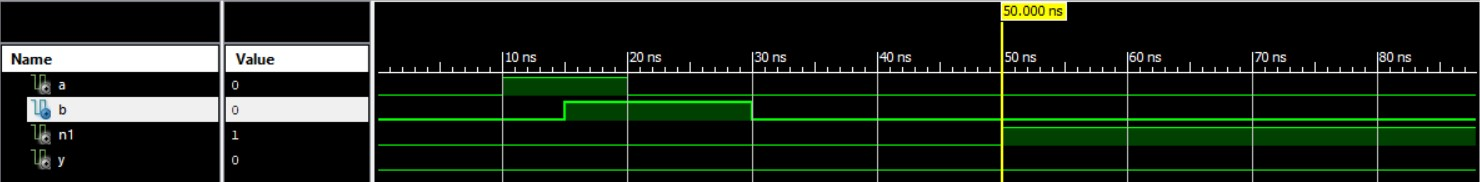
\includegraphics[width=15cm]{images/1_a.jpg}
\end{center}

\subsection*{ب}
برای سیگنال $n1$ برای اینکه تغییرات ورودی در خروجی اعمال شود باید سیگنال ورودی به مدت $15ns$ ثبات داشته باشد، چون نوع تاخیر $inertial$ است و از جایی که ورودی اولیه را برای خروجی صفر فرض می کنیم، پس سیگنال $n1$ تاانتها صفر می‌ماند چون سیگنال $a$ هیچ وقت به ثبات $15ns$ ای نمی رسد.

برای سیگنال $n2$ برای اینکه تغییرات ورودی در خروجی اعمال شود باید سیگنال ورودی به مدت $20ns$ ثبات داشته باشد، چون نوع تاخیر $inertial$ است و از جایی که ورودی اولیه را برای خروجی صفر فرض می کنیم، پس سیگنال $n2$ پس از $30ns$ یک می شود چون سیگنال های $d, e$ در مدت زمان $10ns$ تا $30ns$ یک هستند.

برای سیگنال $n3$ چون  $n1 or c$ است و $n1=0$ پس همان $c$ است با تاخیر $inertial 4ns$.

برای سیگنال $y$ هم تاخیر $inertial 6ns$ دارد و بطور مشابه سیگنال های قبل به سادگی قابل محاسبه است.


\begin{center}
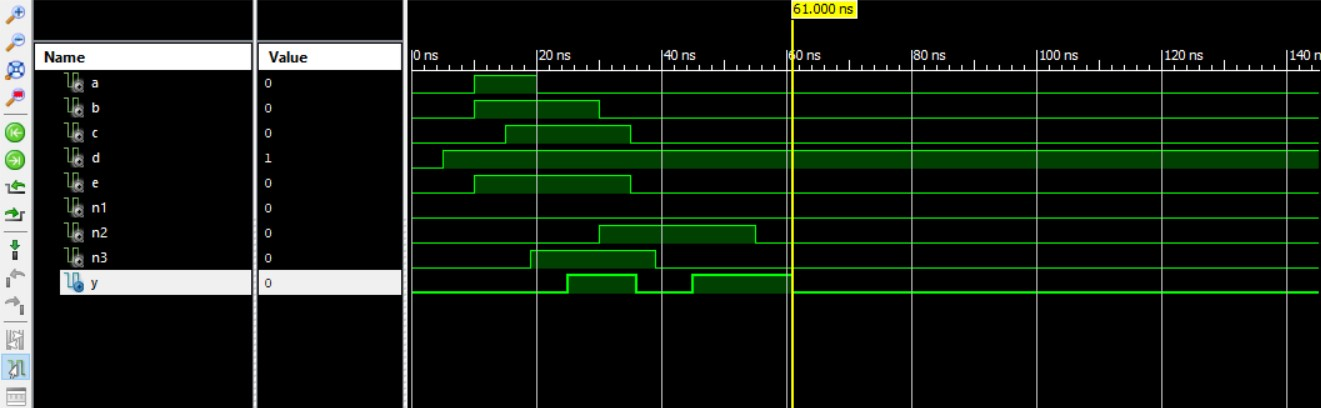
\includegraphics[width=15cm]{images/1_b.jpg}
\end{center}

\newpage
\section{}

\begin{center}
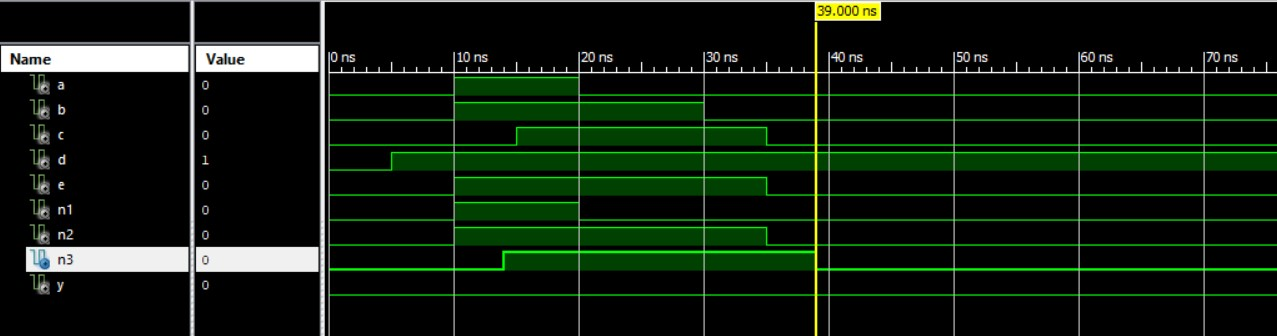
\includegraphics[width=15cm]{images/part2.jpg}
\end{center}

\section{}
\begin{center}
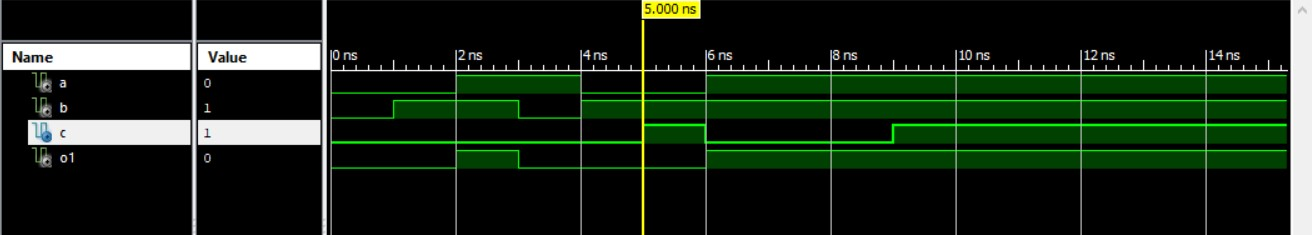
\includegraphics[width=15cm]{images/3_c.jpg}
\end{center}

سیگنال $o1$ را که نتیجه ی بدون تاخیر $ A\land B$ است را رسم می کنیم طبق شکل واضح است که تاخیر $C$ $3ns$ است.

از جایی که مقدار اولیه همه ی ورودی ها طبق فرض صفر است پس تاخیر گیت $not$ برابر $2ns$ است که در $A$ اعمال شده است.

بطور مشابه تاخیر گیت $nand$ $1ns$ است. چون دو ورودی داریم بطور دلخواه $z$ را پس از یک ثانیه یک می گیریم و خروجی برابر نقیض $y$ خواهد بود. سپس در $5ns$ هر دو مقدار را برعکس می کنیم تا صرفا یک $transient$ داشته باشیم.

\begin{center}
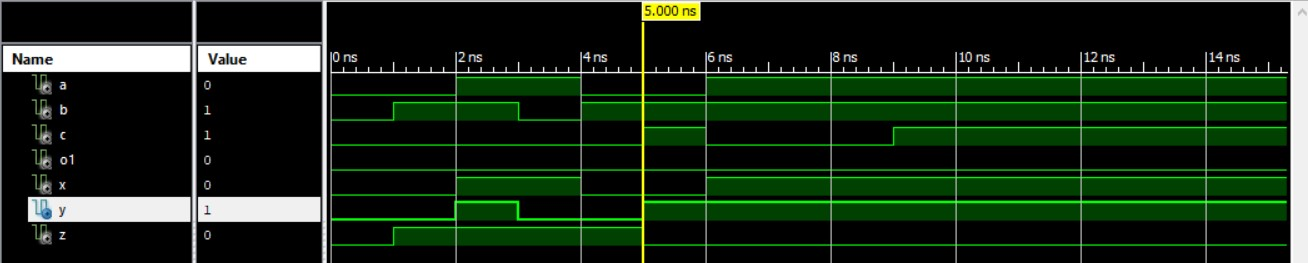
\includegraphics[width=15cm]{images/3.jpg}
\end{center}


\section{}
سیگنال $b$ هر $2ns$ ، $not$ می شود.

سیگنال $a$ یک تاخیر $inertial$ دارد بنابراین برای تغییر خروجی نیاز به $3ns$ ثبات در ورودی ها دارد، پس ابتدا از جایی که $b$ هر $2ns$ تغییر میکند پس نمی تواند تاثیری روی $a$ بگذارد، از طرفی مقدار اولیه $b,a$ صفر است پس سه نانوثانیه صفر می‌ماند و حالا روی خود تاثیر می‌گذارد و به خاطر $nand$ یک می شود و سپس همواره یک می‌ماند. 

\begin{center}
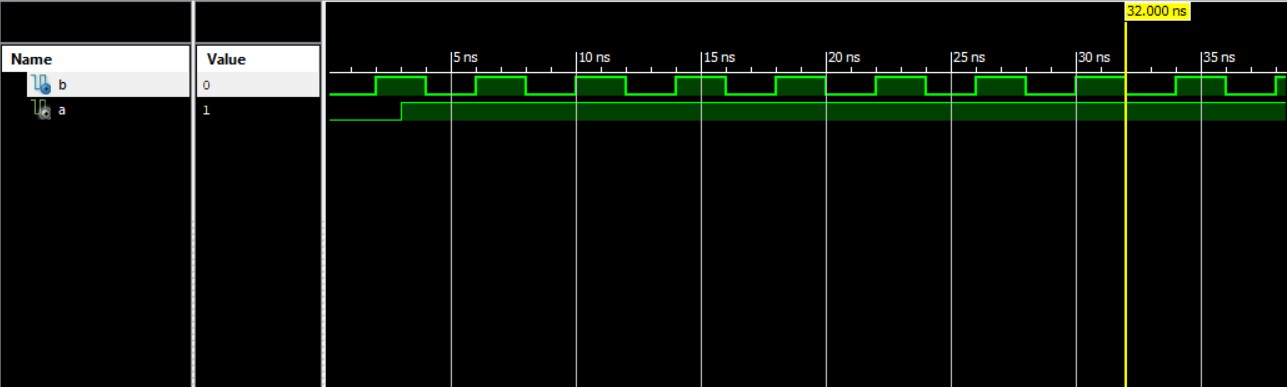
\includegraphics[width=15cm]{images/4.jpg}
\end{center}



\newpage
\goodbye
\end{document}
